
\chapter{Implementation}

\section{Overview}
\section{Design Decisions}

% Efficient Computation
% Updating Dataloaders
% Batched Implementation
% Callbacks
% Training Resumption
% Logging
\section{Proxy Attention}

\begin{algorithm}
    \caption{Single Batch Proxy Attention}
    \label{alg:proxy_attention_single_batch}
    \begin{algorithmic}
        \REQUIRE $input\_wrong$
        \REQUIRE $CAM$
        \REQUIRE $proxy\_threshold$
        \REQUIRE $proxy\_image\_weight$
        \STATE $grads \leftarrow CAM(input\_wrong)$
        \STATE $inversed\_normalized\_inputs \leftarrow inverse\_normalize(input\_wrong)$

        \STATE $output \leftarrow REPLACE(grads \geq proxy\_threshold, ((1- proxy\_image\_weight) * grads) * inversed\_normalized\_inputs, inversed\_normalized\_inputs)$
    \end{algorithmic}
\end{algorithm}


\begin{algorithm}
    \caption{Batch Proxy Attention}
    \label{alg:proxy_attention_batch}
    \begin{algorithmic}
        \REQUIRE $input\_wrong$
        \REQUIRE $label\_wrong$
        \REQUIRE $subset\_chosen$

        \STATE $chosen\_inds = CEIL(subset\_chosen * LENGTH(input\_wrong))$
        \STATE $input\_wrong\_subset = input\_wrong[:chosen_inds]$
        \STATE $label\_wrong\_subset = label\_wrong[:chosen_inds]$

        \STATE $processed\_labels \leftarrow [], processed\_thresholds \leftarrow []$
        \FOR{$i \leftarrow 0$ \TO $LENGTH(label\_wrong\_subset)$}
        \STATE $pass$ \#TODO
        \ENDFOR

    \end{algorithmic}
\end{algorithm}

\section{Challenges and their Potential Solutions}
Being a novel method, there were many challenges that were faced while implementing Proxy Attention. While it was not possible to solve all of the issues faced, the author tried to tackle as many as possible. Many of these issues were posed as optimization problems and were taken into account as hyperparameters that could be tuned to improve performance. This section discusses the possible solutions that were tested. Further details about each parameter can be found in ~\ref{sec:hyperparameters}, while the results of the experiments are discussed in ~\ref{sec:results}.
\subsection{Proxy Method}
The Proxy Attention step involves replacing the pixels in the original images based on the attention maps obtained from a trained model. There are many different ways in which this can be done, some that were explored in the literature, some that were implemented and others that were left for future research. The following are the different methods that were considered:
\subsubsection{Image Statistics Based Replacement}
These methods use either local or global stastistical information from the images for replacement. All these methods can be computed either per image, per batch or over the entire dataset.

\begin{enumerate}
    \item \textbf{Average Pixel Value}: The average pixel value of the original image is used for replacement.
    \item \textbf{Max Pixel Value}: The maximum pixel value of the original image is used for replacement.
    \item \textbf{Min Pixel Value}: The minimum pixel value of the original image is used for replacement.
    \item \textbf{0/255 Pixel Value}: The pixel value of 0 or 255 is used for replacement, where 0 refers to black and 255 refers to white.
\end{enumerate}
These methods are simple, but naive in the sense that they lead to significant information loss. In many cases, if a large number of images have their values replaced with these values, then the model might become biased towards predicting a specific class when an image contains a large number of pixels with these values.
Due to this reason, these methods were not considered for the final implementation.

\subsubsection{Data Augmentation Based Replacement}
Data Augmentation techniques essentially involve computing some transformation over images. Many of these methods were covered in the literature survey ~\ref{sec:augmentation}, some of which replaced the pixels with random values, pixels sampled from either the current image or another image in the dataset, or even deleted the pixels. Most of these methods do not consider the model itself, but some such as Saliency Mix \cite{uddinSaliencyMixSaliencyGuided2021} use measures of saliency to find patches from other images in the dataset that are used to replace the chosen pixels. 
Proxy Attention was inspired by these methods but instead of replacing patches of the image or deleting pixels, it uses a graident based method to downweight the pixels that might have led to the wrong prediction. This method moves away from using naive statistical information but enables the model to eventually learn from the mistakes that it made.

\subsubsection{GAN Based Replacement}


\subsubsection{Modifying the Weights}
Instead of replacing the pixels themselves, another possible method would be to modify the weights of the network directly. While there are many research papers that elaborate on methods to perform this procedure, this domain is not researched enough yet to be used easily. Research on this domain has been done from the early 90s \cite{schmidhuberSelfReferentialWeightMatrix1993}, but practical implementation of such a network that learns to modify its own weight while training have not been extremely successful \cite{irieModernSelfReferentialWeight2022}. 
That being the case, implementing such a method is left to future research. 

\cred{add some papers}

\subsubsection{Multiply with Attention Map}
The method that was chosen for this research does not replace the pixels of the image directly, but weights them using the attention map generated by passing the image through the trained model. 
The obtained attention map is thus multiplied onto the original image. In line with the principles of proxy attention, this is done to allow the network to understand that the parts of the image that it initially focused on did not lead to the correct result. Note that doing so is only possible if the network has seen this image before. Because, after the Proxy Attention step, the images are slightly modified, if the network has not learnt what the original image looks like, it might make more mistakes in the future by learning the wrong set of features.
A caveat of this method is that, after successfully applying the proxy step to a image, the number of pixels that are weighted increases and over time might lead to the image, not having any useful features left. This loss of information is tackled by clearing the proxy images every couple of steps.

\begin{figure}[h]
    \centering
    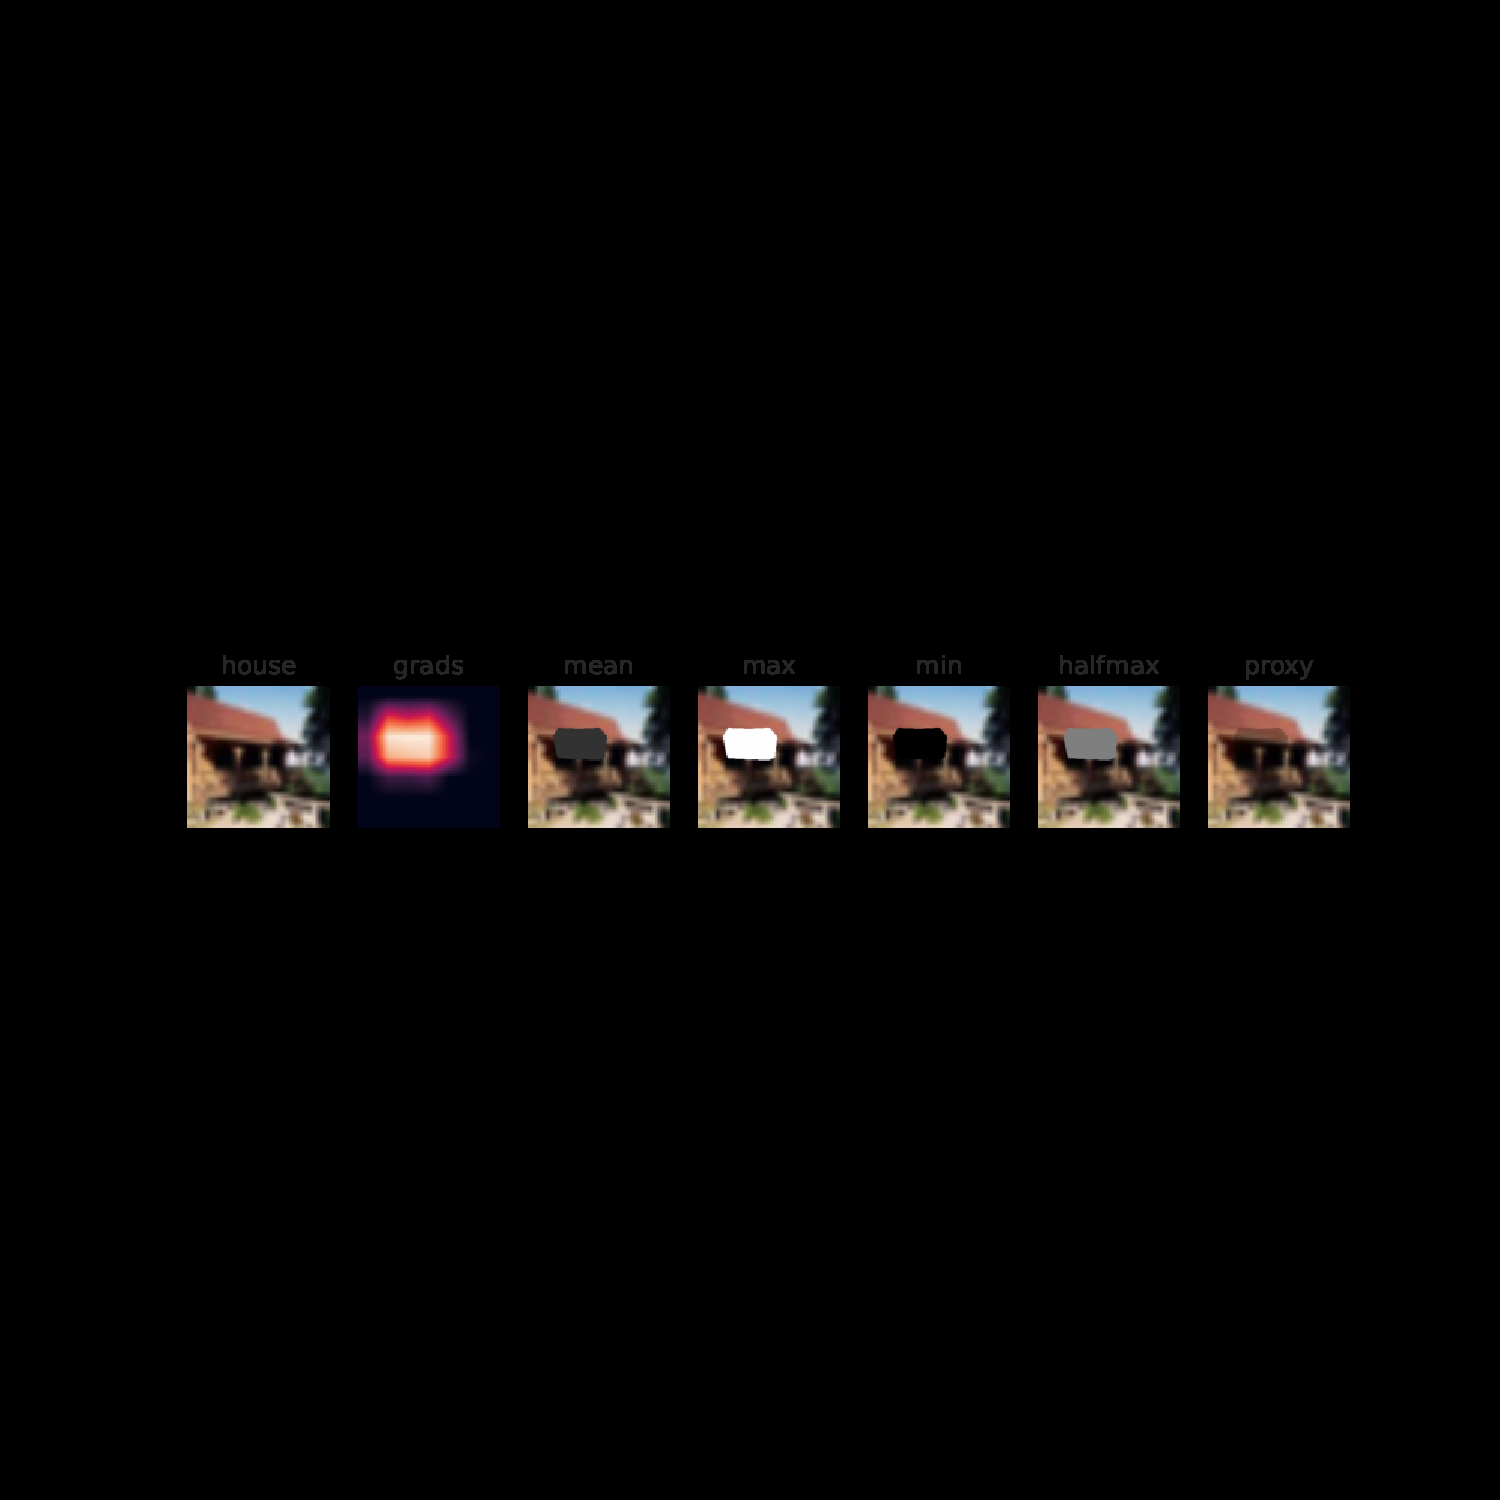
\includegraphics[width=1\textwidth]{images/methods.pdf}
	\caption{Methods}
    \label{fig:methods}
\end{figure}

\subsection{Training Biases}
Gradient based XAI methods are not perfect, and in many cases, they are unable to provide accurate explanations for the predictions made by the model. Since Proxy Attention relies on the outputs of these methods, this might lead to the model learning biased representations of the data. This section discusses the different biases that might be introduced by using these methods in combination with Proxy Attention and how they can potentially be mitigated.

\subsubsection{Method Bias}
Not all explainability methods perform equally, some methods are shown to have better masks generated, while other methods are more computationally expensive. Since Proxy Attention heavily depends on these methods, using them might then lead to additional artefacts in the generated images. It might also be the case that some methods lead to better results while being used alongside proxy attention. To test the effects of this, multiple gradient based methods are used to compare the performance of the networks.

\subsubsection{Mask Bias}
Proxy Attention uses the attention maps produced by gradient based methods and multiplies them on the original image as a mask. While this seems to work well, the masks themselves have edge artefacts that might lead to corrupting some regions of the image. These artefacts are further amplified for smaller image sizes and might impact performance in the log run.
Potential solutions include:

\begin{enumerate}
    \item Smoothing the masks before applying them to the image using techniques such as Eigen Smoothing. This would potentially help in reducing the edge artefacts.
    \item Ensuring that only a certain percentage of the image is replaced by the Proxy Attention step. Doing so would preserve more information. 
\end{enumerate}

\subsubsection{Learning Bias}

\begin{enumerate}
    \item Testing multiple schedules of when to apply the Proxy Attention step. This would help in understanding which part of the training process would benefit from the Proxy Attention step the most, reducing the computational overhead in the long run.
    \item Not reusing previously masked images for the Proxy Step. Doing so ensures that the artefacts are not propagated further into the training process.
\end{enumerate}

\subsubsection{Dataset Bias}

\subsection{Hyper Parameters} \label{sec:hyperparameters}

\subsubsection{Gradient Method}
There are many gradient based methods that are available for generating attention maps from trained networks. While many of these methods were mentioned in the survey, it was not possible to test all of them. Since the effectiveness of Proxy Attention depends quite a bit on the gradient method used, it was important to test them.

The important factor that was considered while choosing these methods was the difference in complexity and the power of explanation that they provide. While algorithms like GradCAM++ \cite{chattopadhayGradCAMGeneralizedGradientBased2018} provide more nuanced and better explanations of the image, older algorithms like Vanilla Gradients \cite{zeilerVisualizingUnderstandingConvolutional2013} are not so accurate. The objective here was to understand if using a more powerful method would improve performance with respect to classification accuracy when used with Proxy Attention. If this indeed is the case, then it would be possible to use more powerful methods to further improve performance in the future.
The gradient methods that were tested are as \cred{follows}:
\begin{itemize}
    \item \textbf{GradCAM++} \cite{chattopadhayGradCAMGeneralizedGradientBased2018}.
    \item \textbf{GradCAM} \cite{selvarajuGradCAMVisualExplanations}
\end{itemize}

\subsubsection{Gradient Threshold Considered}
Every gradient method considered results in the generation of a heatmap where the higher the activation, the more important the pixel is. The activations are mapped to a range of $[0,1]$ with higher values in the heatmap indicating higher activation values. Since using Proxy Attention would mean that the pixels with the chosen activation values would be downweighted, it was important to choose a threshold value that would result in the best classification accuracy.

This is a balancing act as choosing too small of a threshold would result in larger parts of the image being downweighted, while choosing too large of a threshold would result in the image being downweighted too little and hence being too close to the original image to make any difference.

\begin{figure}[h]
    \centering
    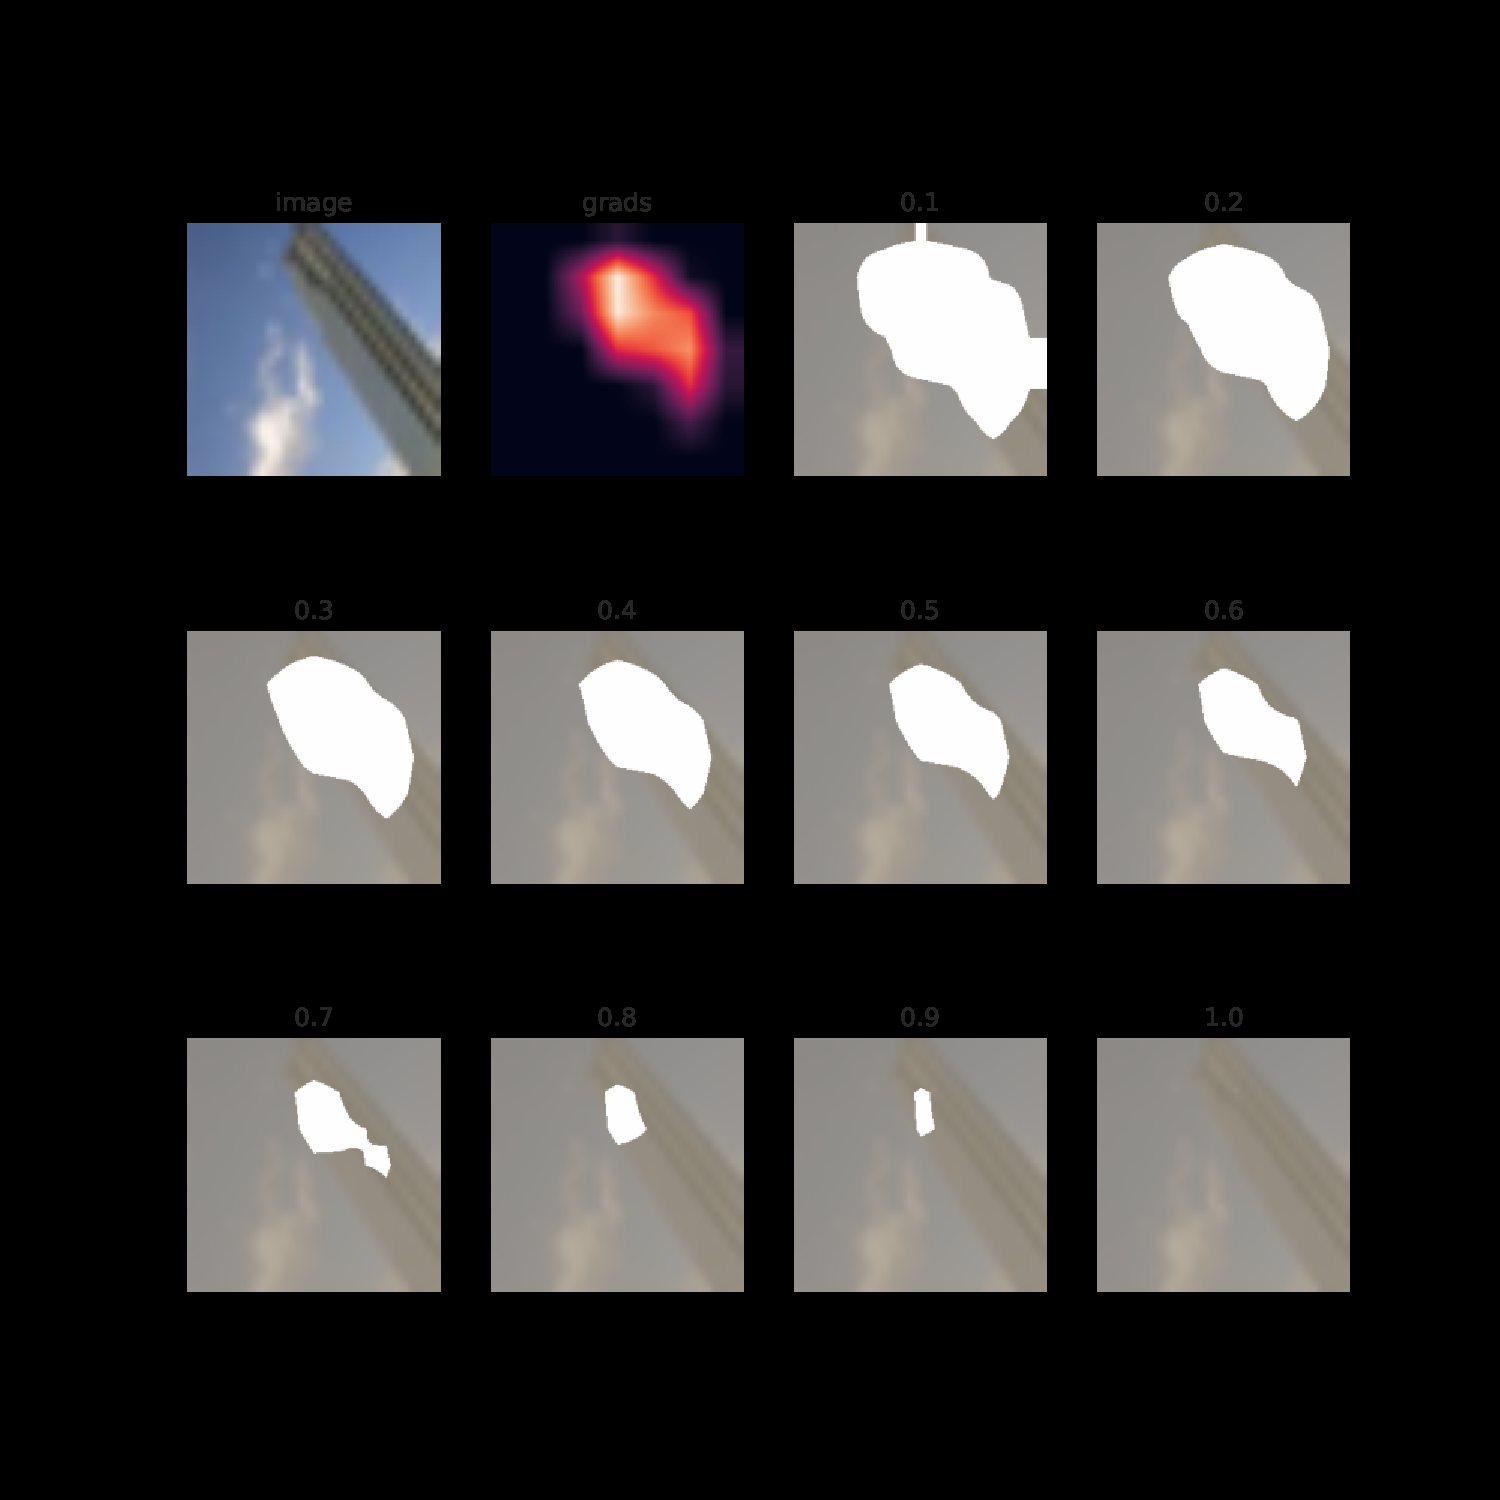
\includegraphics[width=0.8\textwidth]{images/grad_threshold.pdf}
	\caption{Gradient Thresholds}
    \label{fig:thresholds}
\end{figure}

\subsubsection{Multiply Weight}

\subsubsection{Proxy Step Schedule}

\subsubsection{Subset Of Wrongly Classified}

\section{Data Loading and Pre Processing}
\subsection{Directory structure}

\subsection{Label function}

\subsection{Workers}

% Num workers
\subsection{Clearing proxy images} \label{sec:clearing_proxy_images}
For every iteration of the proxy attention step, the images are saved locally. That being the case, it is possible to use these generated images over further iterations of the proxy attention step. Since these images are replacement over the original image from the data set, it is possible to use these images as a direct substitute for the original images in the data set. Note that doing so would lead to the network being given more images in the case of using Proxy Attention during training, which is potentially an unfair comparison. To avoid this issue, only a single image is chosen during the data loading process. This thus becomes a hyper parameter where the options are either to store the last generated proxy images across iterations and use those images as direct replacements for the original images or to not perform the step. 

In the long run, the option to persist the images across iterations might potentially lead to the network learning artefacts that were introduced in prior iterations. To make sure that the networks that train with Proxy Attention are fairly compared with the ones that do not, the data loader is only passed either the original image or it's substitute but not both. 

\subsection{Splits}

\subsection{Augmentations}
Imagenet Normalize
Tensor

\section{Architectures}
TIMM

\section{Grid Search}
To test the effectiveness of Proxy Attention and to find the best combination of hyper parameters, a grid search was performed. The grid search was performed on a single machine with a single GPU and an analysis script was written to determine what trials to run instead of using a separate optimization framework (Ref ~\ref{sec:result_aggregation}). 
Due to limited resources, an intial sweep over the hyperparameters was performed using a low memory network (ResNet18 \cite{heDeepResidualLearning2016}), a subset of the Dogs dataset (\cite{khoslaNovelDatasetFineGrained}), a simple graident method (GradCAM \cite{selvarajuGradCAMVisualExplanations}) and a small number of epochs. A separate process was started for each trial in the grid search and the memory was cleared after each trial. This process was repeated until the best combination of hyper parameters was found. Once the worst performing parameters were eliminated, the rest of the trials were run for the other networks, datasets and methods.
Although it was possible to use a separate optimization framework and an algorithm like Bayesian Optimization to find the best combination of hyper parameters, due to lack of resources and time, the parameters were semi-manually chosen instead.


\section{Training Resumption}
This project required quite a few experiments to be performed to find the best combination of hyper parameters. Due to limitations in the amount of time and resources available, it was important to be able to resume training in case of any interruptions. The author intially tried using libraries such as \href{https://github.com/optuna/optuna}{Optuna} and \href{https://github.com/ray-project/ray}{Ray Tune} but these did not play well on a single machine. (Ref ~\ref{sec:challenges_with_external_libraries}) Considering the scope of this project, a custom solution was implemented instead.

\subsection{Checkpoints} \label{sec:checkpoints}
While checkpoints are almost always a good idea to have, they were especially important in this project. The Proxy Attention step is applied in between training runs and to preserve memory it unloads the existing models and DataLoaders from the GPU. This means that when continuing training, the models and DataLoaders need to be reloaded before the next training run. Doing so would effectively reset the training process and so it was important to have checkpoints to resume training from.
As part of the final analysis, the author also iterated over the trained models and compared the explainability of models trained with or without Proxy Attention. Having saved checkpoints made this process much easier.

\subsection{Broken Trials}
Another challenge of training on a single machine was that the training process could be interrupted at any time. Since multiple trials were being run, it was important to be able to reload the last configuration and continue training from there. The trials were generated as a list of possible configurations and the author iterated over the list to run the trials. If the trail broke, the list of configurations and position of the current trial in the list was saved as a pickled dictionary. Using this saved object, the author could reload the last configuration and continue training easily.

\subsection{Challenges with External Libraries} \label{sec:challenges_with_external_libraries}
Some of the challenges that were faced while using external libraries are as follows:
\begin{enumerate}
    \item \textbf{GPU cache} : While Ray Tune and Optuna do manage resources efficiently, they did not clear the GPU cache effectively. PyTorch by default holds on to the GPU cache and does not release it until the program is closed for efficiency. This would not be a problem for a single training run but many trials were being run, the cache would quickly fill up and cause the training to crash. This does not imply that using Proxy Attention makes it impossible to use such libraries, but that it was easier to implement a custom solution.
    \item \textbf{Cluster} : Both of these libraries were written to enable running large scale experiments over multiple machines. While this would be useful for a large scale project, it added unnecessary complexity for this project as all the experiments were run on a single machine.
    \item \textbf{Grid Search} : Both of the libraries mentioned above were designed to be used for hyper parameter tuning and they implement multiple variants of grid search. While this would be useful, it would stop a lot of trials that would have eventually been useful to analyze. In this project, it was important to be able to have results for each of the trials and the author could not find a way to disable the default Early Stopping behavior as part of the grid search.
\end{enumerate}

\section{Optimizations}
\subsection{Mixed Precision}
Mixed Precision training \cite{micikeviciusMixedPrecisionTraining2017} involves computing most of the operations in the network in half precision (16 bit) and only using full precision (32 bit) for important operations such as the loss function. This allows for much larger batch sizes, faster training and overall reduced memory usage. Micikevicius et al. also find that using Mixed Precision training does not significantly affect the accuracy of the model. With all of these benefits, using Mixed Precision training was a no brainer for this project.

The only caveat is that not all operations are yet stable in half precision. Operations like Batch Normalization tend to break when using Mixed Precision training and unless managed, the model fails to converge. PyTorch supports \href{https://pytorch.org/docs/stable/notes/amp_examples.html}{automatic casting} to and from half precision and this API was used for this project. It is also a registered issue that Transformer models sometimes fail to converge with Mixed Precision due to the way that Attention is calculated (Ref ~\href{https://github.com/pytorch/pytorch/issues/40497}{PyTorch Issue \#40497}), and so for the Vision Transformer \cite{dosovitskiyImageWorth16x162021} model, the author had to use full precision.
\subsection{No grad}
\subsection{Batched Proxy step}

\section{Tensorboard}
Tensorboard is a utility for managing and visualizating training logs. In this project, it is used to store the training configurations, metrics, images and other information that is generated during training. Since Tensorboard uses a custom file format to store this information, it can be used to store any kind of information. Unlike a lot of other logging utilities, Tensorboard stores all it's logs locally. While storing them online might be useful in some cases, it is more difficult to manage and quite unnecessary for this project. 
Another useful feature of Tensorboard is the ability to see live updates while training is in progress. This is useful for debugging and making sure that the training is progressing as expected.


\section{Optimizer}
\section{LR scheduler}
\section{Loss function}
\section{Batch Size Finder}
To maximize training performance, a batch size finder \ref{alg:batch_size_finder} is used to find the optimal batch size for each of the models.

The batch size finder algorithm is rather simple. It is starts off by testing for a small batch size of 2. This batch size is then successively, either incremented, or decremented based on the ability of the current GPU configuration to be able to support that batch of data. 
A random batch of data with the size that is to be tested is generated and is passed through the required model. The rest of the steps required to train a network are also performed on this randomly generated data. If the GPU fails to accommodate the current batch of data, the loop terminates and the required batch size is obtained.
This algorithm remains the same for any model, any data type, any other further optimisations applied (such as mixed precision training \cite{micikeviciusMixedPrecisionTraining2017}), and is robust to multiple GPUs being used for training.
\begin{algorithm}
    \caption{Batch Size Finder Algorithm}
    \label{alg:batch_size_finder}
    \begin{algorithmic}
        \REQUIRE $dataset\_size$
        \REQUIRE $max\_batch\_size$
        \STATE $batch\_size \leftarrow 2$
        \WHILE{TRUE}
        \IF{$max\_batch\_size$ is not $None$ $\And$ $batch\_size \geq max\_batch\_size$}
        \STATE $batch\_size \leftarrow max\_batch\_size$
        \ENDIF
        \IF{$batch\_size \geq dataset\_size$}
        \STATE $batch\_size \leftarrow batch\_size // 2$
        \ENDIF

        \IF{$failed$ is $False$}
        \LOOP
        \STATE $inputs \leftarrow random((batch\_size,input\_shape))$
        \STATE $targets \leftarrow random((batch\_size,output\_shape))$
        \STATE $outputs \leftarrow model(inputs)$
        \STATE $loss \leftarrow MSE(outputs, targets)$
        \STATE $loss.backward()$
        \STATE $optimizer.step()$
        \STATE $optimizer.zero\_grad()$
        \STATE $failed \leftarrow True$
        \STATE $batch\_size \leftarrow batch\_size * 2$
        \ENDLOOP
        \ELSIF{$failed$ is $True$}
        \STATE $failed \leftarrow False$
        \STATE $batch\_size \leftarrow batch\_size // 2$
        \ENDIF

        \ENDWHILE

    \end{algorithmic}
\end{algorithm}

\section{Result Aggregation} \label{sec:result_aggregation}
The biggest caveat of using Tensorboard is that the logs it generates cannot be directly queried in the interface itself. To overcome this, a custom script was written to query the logs and generate a DataFrame that combines all the logs into a single pandas DataFrame. This makes it possible to not only query the logs, but also to perform any kind of analysis on them. Specific queries such as "What is the best accuracy across all the networks for 'gradcam++', 'dogs dataset' and 'proxy\_threshold = 0.5'?" can be easily answered using this script. This makes it possible to easily compare the performance of different models and different configurations. 

Since the script for aggregating logs is rather useful, it was made publicly available as a \href{https://gist.github.com/SubhadityaMukherjee/58cbdf324812175233e91993b720e0bc}{Github Gist}.

\section{Inference}
Inference refers to using a trained model to make predictions on new data. In this project, a large number of models were trained. To be able to use any of the previously trained models for inference, a separate script was created.\\
This script follows from the result aggregation, and can use queries over the dataframe generated in the previous step. Since the generated dataframe also contains the path to the saved model, this script can use that information along with the names of the architecture, dataset and other hyper-parameters to load the required models easily. 
The inference script also contains functions for comparing both the accuracies and the explainability of two pre-trained models given a validation dataset or a list of images.\\
For a batch of images, and given a set of hyperparameters, the script loads two models - one trained with Proxy Attention, and one trained without. The same dataloader is passed through both models to obtain predictions. To ensure fair comparison, only GradCAM++ is used for this evaluation phase. 